\section{Results}

\begin{figure*}

  \begin{panel}{(a)}{\textwidth}
    \def\histogramcsv{figures/data/sim_counting/intensity_histogram.csv}
    \def\tracecsv{figures/data/sim_counting/trace_and_fit_N10.csv}
    \def\traceintensitycol{trace}
    \def\zcol{fit}
    \def\histbincol{N10_bins}
    \def\histcountcol{N10_measured}
    \def\modelfitcol{N10_model}
    \def\posteriorcsv{figures/data/sim_counting/posteriors.csv}
    \def\posteriorcol{posterior_10}
    \hspace{-2mm}
    \tikzsetnextfilename{figure_2_trace_N10}
    \begin{tikzpicture}
      \node (fancyplot) {\begin{tikzpicture}%
  \begin{axis}[
    name=trace,
    width=0.8\textwidth,
    height=5cm,
    xlabel=frames,
    ylabel=intensity,
    enlarge x limits=false,
    xtick distance=500,
    grid=major,
    grid style={dashed},
    scaled ticks=false,
    ticklabel style={font=\small},
    legend style={nodes={scale=0.6, transform shape}},
  ]

    \addplot [
      color=tracecolor,
      mark=*,
      mark size=0.7pt,
      mark options={line width=0},
      fill opacity=0.8,
      draw opacity=0.2,
    ] table [
      col sep=comma,
      x=frames,
      y=\traceintensitycol
    ] {\tracecsv};
    \addlegendentry{intensity trace}

    \addplot [
      color=ztracecolor,
      thick
    ] table [
      col sep=comma,
      x=frames,
      y=\zcol
    ] {\tracecsv};
    \addlegendentry{inferred state}

    % remember min/max y-axis values for next plot
    \pgfplotsextra{
      \pgfmathparse{\pgfkeysvalueof{/pgfplots/ymin}}
      \global\let\ymin\pgfmathresult
      \pgfmathparse{\pgfkeysvalueof{/pgfplots/ymax}}
      \global\let\ymax\pgfmathresult
    }

  \end{axis}

  \begin{axis}[
    at={($(trace.east) + (4mm,0)$)},
    anchor=west,
    width=0.3\textwidth,
    height=5cm,
    yticklabel=\empty,
    xtick distance=0.005,
    xlabel=probability,
    grid=major,
    grid style={dashed, very thin},
    enlarge x limits={value=0.1,upper},
    scaled ticks=false,
    ymin=\ymin,
    ymax=\ymax,
    ticklabel style={font=\small},
    legend style={nodes={scale=0.6, transform shape}},
  ]

    \addplot+[
      xbar interval,
      mark=none,
      color=tracecolor,
      fill=tracecolor,
      fill opacity=0.6,
      draw=none,
    ] table [
      col sep=comma,
      y=\histbincol,
      x=\histcountcol,
    ] {\histogramcsv};
    \addlegendentry{intensity histogram}

    \addplot[
      color=intensitymodelcolor!80!black,
      thick
    ] table [
      col sep=comma,
      y=\histbincol,
      x=\modelfitcol
    ] {\histogramcsv};
    \addlegendentry{inferred model}

  \end{axis}
\end{tikzpicture}%
};
      \def\noylabels{}
      \def\noxlabel{}
      \node[anchor=south east,text width=12mm]
        at ($(fancyplot.south east)+(-0.6,0.8)$)
        {\@ifundefined{noylabels}{}{%
  \pgfplotsset{yticklabel=\empty}%
}%
\begin{tikzpicture}%

  \def\eps{0.001}

  \begin{axis}[
    width=\textwidth,
    height=\textwidth,
    xlabel=\n,
    xlabel=$p(\n|\trace)$,
    grid=major,
    grid style={dashed, very thin},
    enlarge x limits=0.1,
    enlarge y limits=0,
    ymin=0,
    ymax=1,
    scaled ticks=false,
    ticklabel style={font=\small},
  ]

    \addplot+[
      ybar,
      bar width=1,
      mark=none,
      fill=posteriorcolor,
      fill opacity=0.6,
      draw=posteriorcolor,
      y filter/.expression={
        y < \eps ? nan : y
      },
    ] table [
      col sep=comma,
      y=\posteriorcol,
      x=n,
    ] {\posteriorcsv};

    \ifdefined\posteriorcolextra
      \addplot+[
        ybar,
        bar width=1,
        mark=none,
        fill=posteriorcolor!60!black,
        fill opacity=0.6,
        draw=posteriorcolor,
        y filter/.expression={
          y < \eps ? nan : y
        },
      ] table [
        col sep=comma,
        y=\posteriorcolextra,
        x=n,
      ] {\posteriorcsv};
    \fi

  \end{axis}

\end{tikzpicture}
};
    \end{tikzpicture}

    \vspace{-4mm}
  \end{panel}

  \begin{panel}{(b)}{\textwidth}
    \def\histogramcsv{figures/data/sim_counting/intensity_histogram.csv}
    \def\tracecsv{figures/data/sim_counting/trace_and_fit_N20.csv}
    \def\traceintensitycol{trace}
    \def\zcol{fit}
    \def\histbincol{N20_bins}
    \def\histcountcol{N20_measured}
    \def\modelfitcol{N20_model}
    \def\posteriorcsv{figures/data/sim_counting/posteriors.csv}
    \def\posteriorcol{posterior_20}
    \hspace{-2mm}%
    \tikzsetnextfilename{figure_2_trace_N20}
    \begin{tikzpicture}
      \node (fancyplot) {\begin{tikzpicture}%
  \begin{axis}[
    name=trace,
    width=0.8\textwidth,
    height=5cm,
    xlabel=frames,
    ylabel=intensity,
    enlarge x limits=false,
    xtick distance=500,
    grid=major,
    grid style={dashed},
    scaled ticks=false,
    ticklabel style={font=\small},
    legend style={nodes={scale=0.6, transform shape}},
  ]

    \addplot [
      color=tracecolor,
      mark=*,
      mark size=0.7pt,
      mark options={line width=0},
      fill opacity=0.8,
      draw opacity=0.2,
    ] table [
      col sep=comma,
      x=frames,
      y=\traceintensitycol
    ] {\tracecsv};
    \addlegendentry{intensity trace}

    \addplot [
      color=ztracecolor,
      thick
    ] table [
      col sep=comma,
      x=frames,
      y=\zcol
    ] {\tracecsv};
    \addlegendentry{inferred state}

    % remember min/max y-axis values for next plot
    \pgfplotsextra{
      \pgfmathparse{\pgfkeysvalueof{/pgfplots/ymin}}
      \global\let\ymin\pgfmathresult
      \pgfmathparse{\pgfkeysvalueof{/pgfplots/ymax}}
      \global\let\ymax\pgfmathresult
    }

  \end{axis}

  \begin{axis}[
    at={($(trace.east) + (4mm,0)$)},
    anchor=west,
    width=0.3\textwidth,
    height=5cm,
    yticklabel=\empty,
    xtick distance=0.005,
    xlabel=probability,
    grid=major,
    grid style={dashed, very thin},
    enlarge x limits={value=0.1,upper},
    scaled ticks=false,
    ymin=\ymin,
    ymax=\ymax,
    ticklabel style={font=\small},
    legend style={nodes={scale=0.6, transform shape}},
  ]

    \addplot+[
      xbar interval,
      mark=none,
      color=tracecolor,
      fill=tracecolor,
      fill opacity=0.6,
      draw=none,
    ] table [
      col sep=comma,
      y=\histbincol,
      x=\histcountcol,
    ] {\histogramcsv};
    \addlegendentry{intensity histogram}

    \addplot[
      color=intensitymodelcolor!80!black,
      thick
    ] table [
      col sep=comma,
      y=\histbincol,
      x=\modelfitcol
    ] {\histogramcsv};
    \addlegendentry{inferred model}

  \end{axis}
\end{tikzpicture}%
};
      \def\noylabels{}
      \def\noxlabel{}
      \node[anchor=south east,text width=12mm]
        at ($(fancyplot.south east)+(-0.6,0.8)$)
        {\@ifundefined{noylabels}{}{%
  \pgfplotsset{yticklabel=\empty}%
}%
\begin{tikzpicture}%

  \def\eps{0.001}

  \begin{axis}[
    width=\textwidth,
    height=\textwidth,
    xlabel=\n,
    xlabel=$p(\n|\trace)$,
    grid=major,
    grid style={dashed, very thin},
    enlarge x limits=0.1,
    enlarge y limits=0,
    ymin=0,
    ymax=1,
    scaled ticks=false,
    ticklabel style={font=\small},
  ]

    \addplot+[
      ybar,
      bar width=1,
      mark=none,
      fill=posteriorcolor,
      fill opacity=0.6,
      draw=posteriorcolor,
      y filter/.expression={
        y < \eps ? nan : y
      },
    ] table [
      col sep=comma,
      y=\posteriorcol,
      x=n,
    ] {\posteriorcsv};

    \ifdefined\posteriorcolextra
      \addplot+[
        ybar,
        bar width=1,
        mark=none,
        fill=posteriorcolor!60!black,
        fill opacity=0.6,
        draw=posteriorcolor,
        y filter/.expression={
          y < \eps ? nan : y
        },
      ] table [
        col sep=comma,
        y=\posteriorcolextra,
        x=n,
      ] {\posteriorcsv};
    \fi

  \end{axis}

\end{tikzpicture}
};
    \end{tikzpicture}
  \end{panel}

  \begin{panel}{(c)}{0.45\textwidth}
    \def\posteriormatrixcsv{figures/data/sim_counting/heatmap.csv}
    \def\lbfcscsv{figures/data/sim_counting/heatmap_lbfcs.csv}
    \tikzexternaldisable
    \tikzsetnextfilename{figure_2_lbfcs_comparison}
    \begin{tikzpicture}
  \begin{axis}[
    name=trace,
    width=\textwidth,
    height=\textwidth,
    xlabel=Estimated \n,
    ylabel=True \n,
    enlarge x limits=false,
    enlarge y limits=false,
    grid=major,
    grid style={dashed},
    scaled ticks=false,
    ticklabel style={font=\small},
    xtick align=outside,
    xtick pos=lower,
    ytick align=outside,
    ytick pos=lower,
    colorbar,
  ]

    \pgfplotsset{
      colormap={posteriorcolormap}{
        color(0.0)=(white)
        color(0.2)=(funkey_color_2)
        color(1.0)=(funkey_color_2!50!black)
      }
    }

    \addplot[
      matrix plot*,
      mesh/cols=35,
      point meta=explicit,
    ] table [
      col sep=comma,
      x=n,
      y=true_n,
      meta=posterior,
    ] {\posteriormatrixcsv};

  \end{axis}

  \begin{axis}[
    name=trace,
    width=\textwidth,
    height=\textwidth,
    xmin=0.5,
    xmax=35.5,
    ymin=0.5,
    ymax=30.5,
    grid=major,
    grid style={dashed},
    scaled ticks=false,
    domain=0:35,
    ticklabel style={font=\small},
  ]

    \addplot[
      mark=*,
      only marks,
      mark size=1.4pt,
      mark options={draw=white,fill=funkey_color_1,draw opacity=0.6,fill opacity=0.7},
    ] table [
      col sep=comma,
      x=lbfcs_count,
      y=n,
    ] {\lbfcscsv};

    \addplot[no marks,thick,gray] {x};

  \end{axis}

\end{tikzpicture}

    \tikzexternalenable
  \end{panel}
  \hspace{1cm}
  \begin{panel}{(d)}{0.5\textwidth}
    \begin{panel}{}{\textwidth}
      \vspace{2mm}
      \hspace{2mm}
      \small
      \def\tracelengthcsv{figures/data/trace_length/trace_length_results.csv}
      \def\mapcol{max_likelihoods_20}
      \def\varcol{variance_20}
      \tikzexternaldisable
      \tikzsetnextfilename{figure_2_trace_length}
      \def\intervalplot#1#2{%
  \addplot[%
    color=#2,%
    very thick,%
  ] table [%
    col sep=comma,%
    x=length,%
    y=max_likelihoods_#1,%
  ] {\tracelengthcsv};%
  \addplot[%
    name path=lower,%
    draw=none,%
    fill=none,%
    forget plot,%
  ] table [%
    col sep=comma,%
    x=length,%
    y expr=\thisrow{max_likelihoods_#1} - \thisrow{variance_#1}%
  ] {\tracelengthcsv};%
  \addplot[%
    name path=upper,%
    draw=none,%
    fill=none,%
    forget plot,%
  ] table [%
    col sep=comma,%
    x=length,%
    y expr=\thisrow{max_likelihoods_#1} + \thisrow{variance_#1}%
  ] {\tracelengthcsv};%
  \addplot [%
    color=#2,%
    opacity=0.4,%
    forget plot,%
  ] fill between[of=lower and upper];%
  \addlegendentry{$n=#1$};
}%
\begin{tikzpicture}
  \begin{axis}[
    width=\textwidth,
    height=0.47\textwidth,
    xlabel={length [frames]},
    %ylabel=estimated count,
    enlarge x limits=false,
    enlarge y limits=false,
    xtick distance=4000,
    ytick distance=5,
    ymin=0,
    grid=major,
    grid style={dashed},
    scaled ticks=false,
    ticklabel style={font=\small},
    legend columns=4,
    legend style={nodes={scale=0.6, transform shape}},
  ]
    \intervalplot{20}{funkey_color_1}
    \intervalplot{15}{funkey_color_2}
    \intervalplot{10}{funkey_color_3}
    \intervalplot{5}{funkey_color_4}
  \end{axis}
\end{tikzpicture}%

      \tikzexternalenable
    \end{panel}
    \begin{panel}{(e)}{\textwidth}
      \hspace{2mm}
      \small
      \def\tracelengthcsv{figures/data/trace_length/trace_length_results.csv}
      \def\mapcol{max_likelihoods_20}
      \def\varcol{variance_20}
      \tikzexternaldisable
      \tikzsetnextfilename{figure_2_trace_length}
      \def\intervalplot#1#2{%
  \addplot[%
    color=#2,%
    very thick,%
  ] table [%
    col sep=comma,%
    x=length,%
    y=max_likelihoods_#1,%
  ] {\tracelengthcsv};%
  \addplot[%
    name path=lower,%
    draw=none,%
    fill=none,%
    forget plot,%
  ] table [%
    col sep=comma,%
    x=length,%
    y expr=\thisrow{max_likelihoods_#1} - \thisrow{variance_#1}%
  ] {\tracelengthcsv};%
  \addplot[%
    name path=upper,%
    draw=none,%
    fill=none,%
    forget plot,%
  ] table [%
    col sep=comma,%
    x=length,%
    y expr=\thisrow{max_likelihoods_#1} + \thisrow{variance_#1}%
  ] {\tracelengthcsv};%
  \addplot [%
    color=#2,%
    opacity=0.4,%
    forget plot,%
  ] fill between[of=lower and upper];%
  \addlegendentry{$n=#1$};
}%
\begin{tikzpicture}
  \begin{axis}[
    width=\textwidth,
    height=0.47\textwidth,
    xlabel={length [frames]},
    %ylabel=estimated count,
    enlarge x limits=false,
    enlarge y limits=false,
    xtick distance=4000,
    ytick distance=5,
    ymin=0,
    grid=major,
    grid style={dashed},
    scaled ticks=false,
    ticklabel style={font=\small},
    legend columns=4,
    legend style={nodes={scale=0.6, transform shape}},
  ]
    \intervalplot{20}{funkey_color_1}
    \intervalplot{15}{funkey_color_2}
    \intervalplot{10}{funkey_color_3}
    \intervalplot{5}{funkey_color_4}
  \end{axis}
\end{tikzpicture}%

      \tikzexternalenable
    \end{panel}
  \end{panel}

  \caption{
    \panelref{a, b} Trace simulated from 10/20 emitters, and the posterior
    distribution estimated by \ours.
    %
    \panelref{c} The \ours posterior is able to accurately estimate
    significantly higher molecular counts than the current state of the art,
    lbFCS
    %
    \panelref{d} As trace length increases, the variance of the \ours posterior
    decreases.
    %
    \panelref{e} As the signal to noise ratio increases the variance of the
    \ours posterior decreases.
  }
  \label{fig:method:overview}

\end{figure*}

\begin{figure*}

  \begin{panel}{(a)}{0.58\textwidth}
    \small%
    \setlength\plotwidth{42mm}%
    \setlength\plotheight{60mm}%
    \begin{tikzpicture}
  \begin{axis}[
    width=\plotwidth,
    height=\plotheight,
    scale only axis=true,
    name=sweep,
    xlabel=\pon,
    ylabel=\poff,
    enlarge x limits=false,
    enlarge y limits=false,
    scaled ticks=false,
    ticklabel style={/pgf/number format/.cd,fixed,precision=3},
    xtick distance=0.04,
    xtick align=outside,
    xtick pos=lower,
    ytick align=outside,
    ytick pos=lower,
    colorbar,
  ]

    \pgfplotsset{
      colormap={posteriorcolormap}{
        color(0.0)=(funkey_color_2!50!white)
        color(0.1)=(funkey_color_2)
        color(0.9)=(funkey_color_1)
        color(1.0)=(funkey_color_1!50!black)
      }
    }

    \addplot[
      matrix plot*,
      mesh/cols=10,
      point meta=explicit,
    ] table [
      col sep=comma,
      x=p_on,
      y=p_off,
      meta=error,
    ] {\kineticsheatmapcsv};

    % highlight qpaint and lbfcs points
    \node[circle,draw=funkey_color_9,thick] (qpaint) at (axis cs:0.01, 0.2) {};
    \node[circle,draw=funkey_color_9,thick] (lbfcs) at (axis cs:0.02, 0.02) {};

  \end{axis}

  \node[anchor=north] (qpaint_zs) at ($(sweep.north east)+(2.8,0)$) {
    \def\zhistogramcsv{figures/data/kinetics_grid/state_histogram.csv}%
    \def\zhistogramcol{qpaint}%
    \def\noylabels{}%
    \setlength\plotwidth{14mm}%
    \setlength\plotheight{16mm}%
    \tikz{\@ifundefined{noylabels}{}{%
  \pgfplotsset{yticklabel=\empty}%
}%
\@ifundefined{noxlabel}{%
  \pgfplotsset{xlabel=\z{}}%
}{%
  \pgfplotsset{xlabel=\empty}%
}%
\begin{axis}[
  width=\plotwidth,
  height=\plotheight,
  scale only axis=true,
  grid=major,
  grid style={dashed, very thin},
  enlarge x limits=0.1,
  enlarge y limits={value=0.2,upper},
  ymin=0,
  scaled ticks=false,
]

  \addplot+[
    ybar,
    bar width=1,
    mark=none,
    fill=ztracecolor,
    fill opacity=0.6,
    draw=ztracecolor,
  ] table [
    col sep=comma,
    y=\zhistogramcol,
    x=bin,
  ] {\zhistogramcsv};

\end{axis}
}%
  };
  \node[fit=(qpaint_zs),inner sep=0,rounded corners,draw=funkey_color_9,thick] (qpaint_box) {};

  \node[anchor=south] (lbfcs_zs) at (sweep.south-|qpaint_zs.south) {
    \def\zhistogramcsv{figures/data/kinetics_grid/state_histogram.csv}%
    \def\zhistogramcol{lbfcs}%
    \def\noylabels{}%
    \setlength\plotwidth{14mm}%
    \setlength\plotheight{16mm}%
    \tikz{\@ifundefined{noylabels}{}{%
  \pgfplotsset{yticklabel=\empty}%
}%
\@ifundefined{noxlabel}{%
  \pgfplotsset{xlabel=\z{}}%
}{%
  \pgfplotsset{xlabel=\empty}%
}%
\begin{axis}[
  width=\plotwidth,
  height=\plotheight,
  scale only axis=true,
  grid=major,
  grid style={dashed, very thin},
  enlarge x limits=0.1,
  enlarge y limits={value=0.2,upper},
  ymin=0,
  scaled ticks=false,
]

  \addplot+[
    ybar,
    bar width=1,
    mark=none,
    fill=ztracecolor,
    fill opacity=0.6,
    draw=ztracecolor,
  ] table [
    col sep=comma,
    y=\zhistogramcol,
    x=bin,
  ] {\zhistogramcsv};

\end{axis}
}%
  };
  \node[fit=(lbfcs_zs),inner sep=0,rounded corners,draw=funkey_color_9,thick] (lbfcs_box) {};

  \draw[funkey_color_3,thick] (qpaint) -- (qpaint-|qpaint_box.west);
  \draw[funkey_color_3,thick] (lbfcs) -- (lbfcs-|lbfcs_box.west);

\end{tikzpicture}

  \end{panel}
  \begin{panel}{(b)}{0.42\textwidth}
    \setlength\plotwidth{56mm}%
    \setlength\plotheight{60mm}%
    \pgfplotsset{/pgf/number format/.cd,fixed,precision=3}%
\begin{tikzpicture}
  \begin{axis}[
    width=\plotwidth,
    height=\plotheight,
    scale only axis=true,
    xlabel=\pon,
    ylabel=\poff,
    grid=major,
    grid style={dashed},
    scaled ticks=false,
    ticklabel style={font=\small},
  ]
    \pgfplotsset{
      colormap={posteriorcolormap}{
        color(0.0)=(funkey_color_7)
        color(0.5)=(funkey_color_2)
        color(1.0)=(funkey_color_1!50!red)
      }
    }

    \addplot[
      patch,
      patch type=rectangle,
      shader=interp,
      draw=black,
      fill opacity=0.4,
    ] table[
      x=pon_mean,
      y=poff_mean,
      point meta=\thisrow{temperature},
    ] {
      pon_mean    pon_var       poff_mean   poff_var      temperature concentration
      0.02813685  8.5348165e-06 0.07232066  9.0882335e-05 25          10
      0.02797574  1.8311839e-05 0.04775255  5.822931e-05  18          10
      0.05270538  6.0997234e-05 0.04954245  4.0005598e-05 18          20
      0.059536304 5.9824146e-05 0.08741606  0.00014375064 25          20

      0.05270538  6.0997234e-05 0.04954245  4.0005598e-05 18          20
      0.059536304 5.9824146e-05 0.08741606  0.00014375064 25          20
      0.07053028  4.2747815e-05 0.10869306  8.929498e-05  25          30
      0.072243474 0.00016735448 0.05488883  0.0012168097  18          30

      0.02797574  1.8311839e-05 0.04775255  5.822931e-05  18          10
      0.05270538  6.0997234e-05 0.04954245  4.0005598e-05 18          20
      0.045684416 6.31415e-05   0.03472516  8.919405e-05  13          20
      0.024452658 2.4062621e-05 0.036942866 4.378218e-05  13          10

      0.05270538  6.0997234e-05 0.04954245  4.0005598e-05 18          20
      0.072243474 0.00016735448 0.05488883  0.0012168097  18          30
      0.052961048 0.00010537513 0.03289487  6.0903745e-05 13          30
      0.045684416 6.31415e-05   0.03472516  8.919405e-05  13          20
    };

    \addplot[
      scatter,
      mark=*,
      only marks,
      point meta=\thisrow{temperature},
      scatter/@pre marker code/.append style={
        /tikz/mark size=\size,
      },
      visualization depends on={\thisrow{concentration} \as \concentration},
      visualization depends on={2+\thisrow{concentration}*0.1 \as \size},
    ] table [
      col sep=comma,
      x=pon_mean,
      y=poff_mean,
    ] {\kineticscsv};

    \coordinate (n_25_10) at (axis cs:0.02813685,0.07232066) {};
    \coordinate (n_18_10) at (axis cs:0.02797574,0.04775255) {};
    \coordinate (n_13_10) at (axis cs:0.024452658,0.036942866) {};
    \coordinate (n_25_20) at (axis cs:0.059536304,0.08741606) {};
    \coordinate (n_18_20) at (axis cs:0.05270538,0.04954245) {};
    \coordinate (n_13_20) at (axis cs:0.045684416,0.03472516) {};
    \coordinate (n_25_30) at (axis cs:0.07053028,0.10869306) {};
    \coordinate (n_18_30) at (axis cs:0.072243474,0.05488883) {};
    \coordinate (n_13_30) at (axis cs:0.052961048,0.03289487) {};

    \begin{pgfonlayer}{background}
      \draw (n_13_10) -- node[pos=0.5,above,sloped] {\tiny10nM} (n_18_10) -- (n_25_10);
      \draw (n_13_20) -- node[pos=0.5,above,sloped] {\tiny20nM} (n_18_20) -- (n_25_20);
      \draw (n_13_30) -- node[pos=0.5,above,sloped] {\tiny30nM} (n_18_30) -- (n_25_30);
      \draw (n_13_10) -- node[pos=0.5,above,sloped] {\tiny$T=13$} (n_13_20) -- (n_13_30);
      \draw (n_18_10) -- node[pos=0.5,above,sloped] {\tiny$T=18$} (n_18_20) -- (n_18_30);
      \draw (n_25_10) -- node[pos=0.5,above,sloped] {\tiny$T=25$} (n_25_20) -- (n_25_30);
    \end{pgfonlayer}
  \end{axis}

\end{tikzpicture}%

  \end{panel}

  \begin{panel}{(c)}{\textwidth}
    \small%
    \setlength\plotwidth{\textwidth}%
    \setlength\plotheight{36mm}%
    \def\tracecsv{figures/data/kinetics_grid/traces.csv}%
\def\traceintensitycol{qpaint_trace}%
\def\zcol{qpaint_fit}%
\def\histogramcsv{figures/data/kinetics_grid/intensity_histogram.csv}%
\def\histbincol{qpaint_bins}%
\def\histcountcol{qpaint_measured}%
\def\modelfitcol{qpaint_model}%
\def\posteriorcsv{figures/data/kinetics_grid/posteriors.csv}%
\def\posteriorcol{qpaint}%
\tikzsetnextfilename{sim_trace_qpaint}%
\begin{tikzpicture}
  \def\plotlabel{$\n = 10$}
  \@ifundefined{nolabels}{
  \pgfplotsset{xlabel=frames}
  \pgfplotsset{ylabel=intensity}
  \pgfplotsset{grid=major}
  \pgfplotsset{grid style={dashed}}
}{
  \pgfplotsset{xticklabel=\empty}
  \pgfplotsset{yticklabel=\empty}
  \pgfplotsset{ticks=none}
  \pgfplotsset{scaled ticks=false}
}
\@ifundefined{histogramcsv}{}{
  \setlength{\plotwidth}{0.73\plotwidth}
}
\begin{axis}[
  name=trace,
  width=\plotwidth,
  height=\plotheight,
  scale only axis=true,
  enlarge x limits=false,
  xtick distance=500,
  ticklabel style={font=\small},
  legend style={fill=black, nodes={scale=0.6, transform shape}},
]

  \addplot [
    color=tracecolor,
    mark=*,
    mark size=0.7pt,
    mark options={line width=0},
    fill opacity=0.8,
    draw opacity=0.0,
  ] table [
    col sep=comma,
    x=frames,
    y=\traceintensitycol
  ] {\tracecsv};
  \@ifundefined{nolabels}{\addlegendentry{intensity trace}}{}

  \@ifundefined{zcol}{}{
    \addplot [
      color=ztracecolor,
      thick
    ] table [
      col sep=comma,
      x=frames,
      y=\zcol
    ] {\tracecsv};
    \@ifundefined{nolabels}{\addlegendentry{inferred state}}{}
  }

  % remember min/max y-axis values for next plot
  \pgfplotsextra{
    \pgfmathparse{\pgfkeysvalueof{/pgfplots/ymin}}
    \global\let\ymin\pgfmathresult
    \pgfmathparse{\pgfkeysvalueof{/pgfplots/ymax}}
    \global\let\ymax\pgfmathresult
  }

\end{axis}
\@ifundefined{plotlabel}{}{
  \node[anchor=north west,rectangle,draw,fill=black] at (trace.north west) {\plotlabel};
}

\@ifundefined{histogramcsv}{}{
  \begin{axis}[
    at={($(trace.east) + (4mm,0)$)},
    name=histogram,
    anchor=west,
    width=0.25\plotwidth,
    height=\plotheight,
    scale only axis=true,
    ylabel=\empty,
    yticklabel=\empty,
    xtick distance=0.01,
    xlabel=probability,
    grid=major,
    grid style={dashed, very thin},
    enlarge x limits={value=0.4,upper},
    scaled ticks=false,
    ymin=\ymin,
    ymax=\ymax,
    ticklabel style={font=\small},
    legend style={fill=black, nodes={scale=0.6, transform shape}},
  ]

    \addplot+[
      xbar interval,
      mark=none,
      color=tracecolor,
      fill=tracecolor,
      fill opacity=0.6,
      draw=none,
    ] table [
      col sep=comma,
      y=\histbincol,
      x=\histcountcol,
    ] {\histogramcsv};
    \addlegendentry{intensity histogram}

    \addplot[
      color=intensitymodelcolor!80!black,
      thick
    ] table [
      col sep=comma,
      y=\histbincol,
      x=\modelfitcol
    ] {\histogramcsv};
    \addlegendentry{inferred model}

  \end{axis}
}

  \def\noylabels{}
  \def\noxlabel{}
  \setlength\plotwidth{0.1\plotwidth}
  \setlength\plotheight{\plotwidth}
  \pgfplotsset{every axis/.style={
    anchor=below south east,
    at={($(histogram.south east)-(2mm,-4mm)$)},
    xtick distance=10
  }}
  \def\eps{0.001}%  skip bars for values below eps
\@ifundefined{noylabels}{}{
  \pgfplotsset{yticklabel=\empty}
  \pgfplotsset{ylabel=\empty}
}
\@ifundefined{noxlabel}{
  \pgfplotsset{xlabel=$n$}
}{
  \pgfplotsset{xlabel=\empty}
}
\begin{axis}[
  width=\plotwidth,
  height=\plotheight,
  scale only axis=true,
  enlarge x limits={abs=1.5},
  enlarge y limits=0,
  ymin=0,
  ymax=1,
  scaled ticks=false,
  ticklabel style={font=\tiny},
  xtick distance=1,
  axis background/.style={fill=white},
]

  \addplot+[
    ybar,
    bar width=1,
    mark=none,
    fill=posteriorcolor,
    fill opacity=0.6,
    draw=posteriorcolor,
    y filter/.expression={
      y < \eps ? nan : y
    },
  ] table [
    col sep=comma,
    y=\posteriorcol,
    x=n,
  ] {\posteriorcsv};

  \ifdefined\posteriorcolextra
    \addplot+[
      ybar,
      bar width=1,
      mark=none,
      fill=posteriorcolor!60!black,
      fill opacity=0.6,
      draw=posteriorcolor,
      y filter/.expression={
        y < \eps ? nan : y
      },
    ] table [
      col sep=comma,
      y=\posteriorcolextra,
      x=n,
    ] {\posteriorcsv};
  \fi

\end{axis}

\end{tikzpicture}
%
    \vspace{-4mm}%
  \end{panel}

  \begin{panel}{(d)}{\textwidth}
    \small%
    \setlength\plotwidth{\textwidth}%
    \setlength\plotheight{36mm}%
    \def\tracecsv{figures/data/kinetics_grid/traces.csv}%
\def\traceintensitycol{lbfcs_trace}%
\def\zcol{lbfcs_fit}%
\def\histogramcsv{figures/data/kinetics_grid/intensity_histogram.csv}%
\def\histbincol{lbfcs_bins}%
\def\histcountcol{lbfcs_measured}%
\def\modelfitcol{lbfcs_model}%
\def\posteriorcsv{figures/data/kinetics_grid/posteriors.csv}%
\def\posteriorcol{lbfcs}%
\tikzsetnextfilename{sim_trace_lbfcs}%
\begin{tikzpicture}
  \def\plotlabel{$\n = 10$}
  \@ifundefined{nolabels}{
  \pgfplotsset{xlabel=frames}
  \pgfplotsset{ylabel=intensity}
  \pgfplotsset{grid=major}
  \pgfplotsset{grid style={dashed}}
}{
  \pgfplotsset{xticklabel=\empty}
  \pgfplotsset{yticklabel=\empty}
  \pgfplotsset{ticks=none}
  \pgfplotsset{scaled ticks=false}
}
\@ifundefined{histogramcsv}{}{
  \setlength{\plotwidth}{0.73\plotwidth}
}
\begin{axis}[
  name=trace,
  width=\plotwidth,
  height=\plotheight,
  scale only axis=true,
  enlarge x limits=false,
  xtick distance=500,
  ticklabel style={font=\small},
  legend style={fill=black, nodes={scale=0.6, transform shape}},
]

  \addplot [
    color=tracecolor,
    mark=*,
    mark size=0.7pt,
    mark options={line width=0},
    fill opacity=0.8,
    draw opacity=0.0,
  ] table [
    col sep=comma,
    x=frames,
    y=\traceintensitycol
  ] {\tracecsv};
  \@ifundefined{nolabels}{\addlegendentry{intensity trace}}{}

  \@ifundefined{zcol}{}{
    \addplot [
      color=ztracecolor,
      thick
    ] table [
      col sep=comma,
      x=frames,
      y=\zcol
    ] {\tracecsv};
    \@ifundefined{nolabels}{\addlegendentry{inferred state}}{}
  }

  % remember min/max y-axis values for next plot
  \pgfplotsextra{
    \pgfmathparse{\pgfkeysvalueof{/pgfplots/ymin}}
    \global\let\ymin\pgfmathresult
    \pgfmathparse{\pgfkeysvalueof{/pgfplots/ymax}}
    \global\let\ymax\pgfmathresult
  }

\end{axis}
\@ifundefined{plotlabel}{}{
  \node[anchor=north west,rectangle,draw,fill=black] at (trace.north west) {\plotlabel};
}

\@ifundefined{histogramcsv}{}{
  \begin{axis}[
    at={($(trace.east) + (4mm,0)$)},
    name=histogram,
    anchor=west,
    width=0.25\plotwidth,
    height=\plotheight,
    scale only axis=true,
    ylabel=\empty,
    yticklabel=\empty,
    xtick distance=0.01,
    xlabel=probability,
    grid=major,
    grid style={dashed, very thin},
    enlarge x limits={value=0.4,upper},
    scaled ticks=false,
    ymin=\ymin,
    ymax=\ymax,
    ticklabel style={font=\small},
    legend style={fill=black, nodes={scale=0.6, transform shape}},
  ]

    \addplot+[
      xbar interval,
      mark=none,
      color=tracecolor,
      fill=tracecolor,
      fill opacity=0.6,
      draw=none,
    ] table [
      col sep=comma,
      y=\histbincol,
      x=\histcountcol,
    ] {\histogramcsv};
    \addlegendentry{intensity histogram}

    \addplot[
      color=intensitymodelcolor!80!black,
      thick
    ] table [
      col sep=comma,
      y=\histbincol,
      x=\modelfitcol
    ] {\histogramcsv};
    \addlegendentry{inferred model}

  \end{axis}
}

  \def\noylabels{}
  \def\noxlabel{}
  \setlength\plotwidth{0.1\plotwidth}
  \setlength\plotheight{\plotwidth}
  \pgfplotsset{every axis/.style={
    anchor=below south east,
    at={($(histogram.south east)-(2mm,-4mm)$)},
    xtick distance=2
  }}
  \def\eps{0.001}%  skip bars for values below eps
\@ifundefined{noylabels}{}{
  \pgfplotsset{yticklabel=\empty}
  \pgfplotsset{ylabel=\empty}
}
\@ifundefined{noxlabel}{
  \pgfplotsset{xlabel=$n$}
}{
  \pgfplotsset{xlabel=\empty}
}
\begin{axis}[
  width=\plotwidth,
  height=\plotheight,
  scale only axis=true,
  enlarge x limits={abs=1.5},
  enlarge y limits=0,
  ymin=0,
  ymax=1,
  scaled ticks=false,
  ticklabel style={font=\tiny},
  xtick distance=1,
  axis background/.style={fill=white},
]

  \addplot+[
    ybar,
    bar width=1,
    mark=none,
    fill=posteriorcolor,
    fill opacity=0.6,
    draw=posteriorcolor,
    y filter/.expression={
      y < \eps ? nan : y
    },
  ] table [
    col sep=comma,
    y=\posteriorcol,
    x=n,
  ] {\posteriorcsv};

  \ifdefined\posteriorcolextra
    \addplot+[
      ybar,
      bar width=1,
      mark=none,
      fill=posteriorcolor!60!black,
      fill opacity=0.6,
      draw=posteriorcolor,
      y filter/.expression={
        y < \eps ? nan : y
      },
    ] table [
      col sep=comma,
      y=\posteriorcolextra,
      x=n,
    ] {\posteriorcsv};
  \fi

\end{axis}

\end{tikzpicture}

  \end{panel}

  \caption{%
    \panelref{a} The counting ability of \ours varies significantly with
    blinking kinetics of the emitters, showing increased model accuracy when
    $\pon > \poff$. Top inset: when $\pon < \poff$, the distribution of
    observed \z{} states is shifted towards 0 (top inset). Bottom inset: for
    $\pon > \poff$, the distribution of \z{} states is shifted towards \n (the
    number of emitters).
    %
    \panelref{b} TODO
    %
    \panelref{c} TODO
    %
    \panelref{d} TODO
  }
  \label{fig:method:overview}
\end{figure*}

\begin{figure*}

  \begin{panel}{(a)}{\textwidth}
    \hspace{-2mm}%
    \setlength\plotwidth{\textwidth}%
    \setlength\plotheight{36mm}%
    \def\histogramcsv{figures/data/qpaint_kinetics/intensity_histogram.csv}%
\def\tracecsv{figures/data/qpaint_kinetics/trace_and_fit_N10.csv}%
\def\traceintensitycol{trace}%
\def\zcol{fit}%
\def\histbincol{N10_bins}%
\def\histcountcol{N10_measured}%
\def\modelfitcol{N10_model}%
\def\posteriorcsv{figures/data/qpaint_kinetics/posteriors.csv}%
\def\posteriorcol{posterior_10}%
\tikzsetnextfilename{qpaint_trace_n10}%
\begin{tikzpicture}
  \@ifundefined{nolabels}{
  \pgfplotsset{xlabel=frames}
  \pgfplotsset{ylabel=intensity}
  \pgfplotsset{grid=major}
  \pgfplotsset{grid style={dashed}}
}{
  \pgfplotsset{xticklabel=\empty}
  \pgfplotsset{yticklabel=\empty}
  \pgfplotsset{ticks=none}
  \pgfplotsset{scaled ticks=false}
}
\@ifundefined{histogramcsv}{}{
  \setlength{\plotwidth}{0.73\plotwidth}
}
\begin{axis}[
  name=trace,
  width=\plotwidth,
  height=\plotheight,
  scale only axis=true,
  enlarge x limits=false,
  xtick distance=500,
  ticklabel style={font=\small},
  legend style={fill=black, nodes={scale=0.6, transform shape}},
]

  \addplot [
    color=tracecolor,
    mark=*,
    mark size=0.7pt,
    mark options={line width=0},
    fill opacity=0.8,
    draw opacity=0.0,
  ] table [
    col sep=comma,
    x=frames,
    y=\traceintensitycol
  ] {\tracecsv};
  \@ifundefined{nolabels}{\addlegendentry{intensity trace}}{}

  \@ifundefined{zcol}{}{
    \addplot [
      color=ztracecolor,
      thick
    ] table [
      col sep=comma,
      x=frames,
      y=\zcol
    ] {\tracecsv};
    \@ifundefined{nolabels}{\addlegendentry{inferred state}}{}
  }

  % remember min/max y-axis values for next plot
  \pgfplotsextra{
    \pgfmathparse{\pgfkeysvalueof{/pgfplots/ymin}}
    \global\let\ymin\pgfmathresult
    \pgfmathparse{\pgfkeysvalueof{/pgfplots/ymax}}
    \global\let\ymax\pgfmathresult
  }

\end{axis}
\@ifundefined{plotlabel}{}{
  \node[anchor=north west,rectangle,draw,fill=black] at (trace.north west) {\plotlabel};
}

\@ifundefined{histogramcsv}{}{
  \begin{axis}[
    at={($(trace.east) + (4mm,0)$)},
    name=histogram,
    anchor=west,
    width=0.25\plotwidth,
    height=\plotheight,
    scale only axis=true,
    ylabel=\empty,
    yticklabel=\empty,
    xtick distance=0.01,
    xlabel=probability,
    grid=major,
    grid style={dashed, very thin},
    enlarge x limits={value=0.4,upper},
    scaled ticks=false,
    ymin=\ymin,
    ymax=\ymax,
    ticklabel style={font=\small},
    legend style={fill=black, nodes={scale=0.6, transform shape}},
  ]

    \addplot+[
      xbar interval,
      mark=none,
      color=tracecolor,
      fill=tracecolor,
      fill opacity=0.6,
      draw=none,
    ] table [
      col sep=comma,
      y=\histbincol,
      x=\histcountcol,
    ] {\histogramcsv};
    \addlegendentry{intensity histogram}

    \addplot[
      color=intensitymodelcolor!80!black,
      thick
    ] table [
      col sep=comma,
      y=\histbincol,
      x=\modelfitcol
    ] {\histogramcsv};
    \addlegendentry{inferred model}

  \end{axis}
}

  \def\noylabels{}
  \def\noxlabel{}
  \setlength\plotwidth{0.1\plotwidth}
  \setlength\plotheight{\plotwidth}
  \pgfplotsset{every axis/.style={anchor=below south east,at={($(histogram.south east)-(2mm,0)$)}}}
  \def\eps{0.001}%  skip bars for values below eps
\@ifundefined{noylabels}{}{
  \pgfplotsset{yticklabel=\empty}
  \pgfplotsset{ylabel=\empty}
}
\@ifundefined{noxlabel}{
  \pgfplotsset{xlabel=$n$}
}{
  \pgfplotsset{xlabel=\empty}
}
\begin{axis}[
  width=\plotwidth,
  height=\plotheight,
  scale only axis=true,
  enlarge x limits={abs=1.5},
  enlarge y limits=0,
  ymin=0,
  ymax=1,
  scaled ticks=false,
  ticklabel style={font=\tiny},
  xtick distance=1,
  axis background/.style={fill=white},
]

  \addplot+[
    ybar,
    bar width=1,
    mark=none,
    fill=posteriorcolor,
    fill opacity=0.6,
    draw=posteriorcolor,
    y filter/.expression={
      y < \eps ? nan : y
    },
  ] table [
    col sep=comma,
    y=\posteriorcol,
    x=n,
  ] {\posteriorcsv};

  \ifdefined\posteriorcolextra
    \addplot+[
      ybar,
      bar width=1,
      mark=none,
      fill=posteriorcolor!60!black,
      fill opacity=0.6,
      draw=posteriorcolor,
      y filter/.expression={
        y < \eps ? nan : y
      },
    ] table [
      col sep=comma,
      y=\posteriorcolextra,
      x=n,
    ] {\posteriorcsv};
  \fi

\end{axis}

\end{tikzpicture}

    \vspace{-4mm}
  \end{panel}

  \begin{panel}{(a)}{\textwidth}
    \hspace{-2mm}%
    \setlength\plotwidth{\textwidth}%
    \setlength\plotheight{36mm}%
    \def\histogramcsv{figures/data/qpaint_kinetics/intensity_histogram.csv}%
\def\tracecsv{figures/data/qpaint_kinetics/trace_and_fit_N20.csv}%
\def\traceintensitycol{trace}%
\def\zcol{fit}%
\def\histbincol{N20_bins}%
\def\histcountcol{N20_measured}%
\def\modelfitcol{N20_model}%
\def\posteriorcsv{figures/data/qpaint_kinetics/posteriors.csv}%
\def\posteriorcol{posterior_20}%
\tikzsetnextfilename{qpaint_trace_n20}%
\begin{tikzpicture}
  \@ifundefined{nolabels}{
  \pgfplotsset{xlabel=frames}
  \pgfplotsset{ylabel=intensity}
  \pgfplotsset{grid=major}
  \pgfplotsset{grid style={dashed}}
}{
  \pgfplotsset{xticklabel=\empty}
  \pgfplotsset{yticklabel=\empty}
  \pgfplotsset{ticks=none}
  \pgfplotsset{scaled ticks=false}
}
\@ifundefined{histogramcsv}{}{
  \setlength{\plotwidth}{0.73\plotwidth}
}
\begin{axis}[
  name=trace,
  width=\plotwidth,
  height=\plotheight,
  scale only axis=true,
  enlarge x limits=false,
  xtick distance=500,
  ticklabel style={font=\small},
  legend style={fill=black, nodes={scale=0.6, transform shape}},
]

  \addplot [
    color=tracecolor,
    mark=*,
    mark size=0.7pt,
    mark options={line width=0},
    fill opacity=0.8,
    draw opacity=0.0,
  ] table [
    col sep=comma,
    x=frames,
    y=\traceintensitycol
  ] {\tracecsv};
  \@ifundefined{nolabels}{\addlegendentry{intensity trace}}{}

  \@ifundefined{zcol}{}{
    \addplot [
      color=ztracecolor,
      thick
    ] table [
      col sep=comma,
      x=frames,
      y=\zcol
    ] {\tracecsv};
    \@ifundefined{nolabels}{\addlegendentry{inferred state}}{}
  }

  % remember min/max y-axis values for next plot
  \pgfplotsextra{
    \pgfmathparse{\pgfkeysvalueof{/pgfplots/ymin}}
    \global\let\ymin\pgfmathresult
    \pgfmathparse{\pgfkeysvalueof{/pgfplots/ymax}}
    \global\let\ymax\pgfmathresult
  }

\end{axis}
\@ifundefined{plotlabel}{}{
  \node[anchor=north west,rectangle,draw,fill=black] at (trace.north west) {\plotlabel};
}

\@ifundefined{histogramcsv}{}{
  \begin{axis}[
    at={($(trace.east) + (4mm,0)$)},
    name=histogram,
    anchor=west,
    width=0.25\plotwidth,
    height=\plotheight,
    scale only axis=true,
    ylabel=\empty,
    yticklabel=\empty,
    xtick distance=0.01,
    xlabel=probability,
    grid=major,
    grid style={dashed, very thin},
    enlarge x limits={value=0.4,upper},
    scaled ticks=false,
    ymin=\ymin,
    ymax=\ymax,
    ticklabel style={font=\small},
    legend style={fill=black, nodes={scale=0.6, transform shape}},
  ]

    \addplot+[
      xbar interval,
      mark=none,
      color=tracecolor,
      fill=tracecolor,
      fill opacity=0.6,
      draw=none,
    ] table [
      col sep=comma,
      y=\histbincol,
      x=\histcountcol,
    ] {\histogramcsv};
    \addlegendentry{intensity histogram}

    \addplot[
      color=intensitymodelcolor!80!black,
      thick
    ] table [
      col sep=comma,
      y=\histbincol,
      x=\modelfitcol
    ] {\histogramcsv};
    \addlegendentry{inferred model}

  \end{axis}
}

  \def\noylabels{}
  \def\noxlabel{}
  \setlength\plotwidth{0.1\plotwidth}
  \setlength\plotheight{\plotwidth}
  \pgfplotsset{every axis/.style={anchor=below south east,at={($(histogram.south east)-(2mm,0)$)}}}
  \def\eps{0.001}%  skip bars for values below eps
\@ifundefined{noylabels}{}{
  \pgfplotsset{yticklabel=\empty}
  \pgfplotsset{ylabel=\empty}
}
\@ifundefined{noxlabel}{
  \pgfplotsset{xlabel=$n$}
}{
  \pgfplotsset{xlabel=\empty}
}
\begin{axis}[
  width=\plotwidth,
  height=\plotheight,
  scale only axis=true,
  enlarge x limits={abs=1.5},
  enlarge y limits=0,
  ymin=0,
  ymax=1,
  scaled ticks=false,
  ticklabel style={font=\tiny},
  xtick distance=1,
  axis background/.style={fill=white},
]

  \addplot+[
    ybar,
    bar width=1,
    mark=none,
    fill=posteriorcolor,
    fill opacity=0.6,
    draw=posteriorcolor,
    y filter/.expression={
      y < \eps ? nan : y
    },
  ] table [
    col sep=comma,
    y=\posteriorcol,
    x=n,
  ] {\posteriorcsv};

  \ifdefined\posteriorcolextra
    \addplot+[
      ybar,
      bar width=1,
      mark=none,
      fill=posteriorcolor!60!black,
      fill opacity=0.6,
      draw=posteriorcolor,
      y filter/.expression={
        y < \eps ? nan : y
      },
    ] table [
      col sep=comma,
      y=\posteriorcolextra,
      x=n,
    ] {\posteriorcsv};
  \fi

\end{axis}

\end{tikzpicture}

    \vspace{-4mm}
  \end{panel}

  \begin{panel}{(c)}{\textwidth}
    \setlength\plotwidth{72mm}%
    \setlength\plotheight{72mm}%
    \def\posteriormatrixcsv{figures/data/qpaint_kinetics/heatmap.csv}%
\def\qpaintcsv{figures/data/qpaint_kinetics/qpaint_counts.csv}%
\tikzsetnextfilename{qpaint_counting_estimates}%
\begin{tikzpicture}
  \begin{axis}[
    name=trace,
    width=\plotwidth,
    height=\plotheight,
    xlabel=true \n,
    ylabel=estimated \n,
    enlarge x limits=false,
    enlarge y limits=false,
    grid=major,
    grid style={dashed},
    scaled ticks=false,
    ticklabel style={font=\small},
    xtick align=outside,
    xtick pos=lower,
    ytick align=outside,
    ytick pos=lower,
    colorbar,
  ]

    \pgfplotsset{
      colormap={posteriorcolormap}{
        color(0.0)=(white)
        color(0.2)=(funkey_color_2)
        color(1.0)=(funkey_color_2!50!black)
      }
    }

    \addplot[
      matrix plot*,
      mesh/cols=30,
      point meta=explicit,
    ] table [
      col sep=comma,
      x=n_true,
      y=n_fit,
      meta=posterior,
    ] {\posteriormatrixcsv};

  \end{axis}

  \begin{axis}[
    name=trace,
    width=\plotwidth,
    height=\plotheight,
    xmin=0.5,
    xmax=30.5,
    ymin=0.5,
    ymax=35.5,
    grid=major,
    grid style={dashed},
    xticklabel=\empty,
    yticklabel=\empty,
    scaled ticks=false,
    domain=0:30,
    ticklabel style={font=\small},
    legend pos=north west,
  ]

    \addlegendimage{mark=square*,only marks,funkey_color_2}
    \addlegendentry{\ours}
    \addlegendimage{mark=*,only marks,funkey_color_1}
    \addlegendentry{\qpaint}

    \addplot[
      mark=*,
      only marks,
      mark size=1.4pt,
      mark options={draw=white,fill=funkey_color_1,draw opacity=0.6,fill opacity=0.7},
    ] table [
      col sep=comma,
      x=n,
      y=qpaint_count,
    ] {\qpaintcsv};

    \addplot[no marks,thick,gray] {x};

  \end{axis}

\end{tikzpicture}

  \end{panel}
  \caption{
    \panelref{a, b} trace simulated with 10/20 emitters, \pon=0.006, \poff=0.2, 
    and the posterior distribution estimated by \ours
    %
    \panelref{c} At higher molecular counts ($n > 15$) \qpaint begins to underestimate the count, while 
    the posterior of \ours remains accurate.
    %
    }
  \label{fig:results:qpaint_counting}
\end{figure*}


\begin{figure*}[t]

  \begin{panel}{(a)}{\textwidth}
    \hspace{-2mm}%
    \setlength\plotwidth{\textwidth}%
    \setlength\plotheight{36mm}%
    \def\histogramcsv{figures/data/exp_counting/intensity_histograms.csv}%
\def\tracecsv{figures/data/exp_counting/traces_and_fits.csv}%
\def\posteriorcsv{figures/data/exp_counting/posteriors.csv}%
\def\traceintensitycol{N1_trace_good}%
\def\zcol{N1_fit_good}%
\def\histbincol{N1_good_bins}%
\def\histcountcol{N1_good_measured}%
\def\modelfitcol{N1_good_model}%
\def\posteriorcol{posterior_1}%
\tikzsetnextfilename{exp_trace_n1}%
\begin{tikzpicture}
  \@ifundefined{nolabels}{
  \pgfplotsset{xlabel=frames}
  \pgfplotsset{ylabel=intensity}
  \pgfplotsset{grid=major}
  \pgfplotsset{grid style={dashed}}
}{
  \pgfplotsset{xticklabel=\empty}
  \pgfplotsset{yticklabel=\empty}
  \pgfplotsset{ticks=none}
  \pgfplotsset{scaled ticks=false}
}
\@ifundefined{histogramcsv}{}{
  \setlength{\plotwidth}{0.73\plotwidth}
}
\begin{axis}[
  name=trace,
  width=\plotwidth,
  height=\plotheight,
  scale only axis=true,
  enlarge x limits=false,
  xtick distance=500,
  ticklabel style={font=\small},
  legend style={fill=black, nodes={scale=0.6, transform shape}},
]

  \addplot [
    color=tracecolor,
    mark=*,
    mark size=0.7pt,
    mark options={line width=0},
    fill opacity=0.8,
    draw opacity=0.0,
  ] table [
    col sep=comma,
    x=frames,
    y=\traceintensitycol
  ] {\tracecsv};
  \@ifundefined{nolabels}{\addlegendentry{intensity trace}}{}

  \@ifundefined{zcol}{}{
    \addplot [
      color=ztracecolor,
      thick
    ] table [
      col sep=comma,
      x=frames,
      y=\zcol
    ] {\tracecsv};
    \@ifundefined{nolabels}{\addlegendentry{inferred state}}{}
  }

  % remember min/max y-axis values for next plot
  \pgfplotsextra{
    \pgfmathparse{\pgfkeysvalueof{/pgfplots/ymin}}
    \global\let\ymin\pgfmathresult
    \pgfmathparse{\pgfkeysvalueof{/pgfplots/ymax}}
    \global\let\ymax\pgfmathresult
  }

\end{axis}
\@ifundefined{plotlabel}{}{
  \node[anchor=north west,rectangle,draw,fill=black] at (trace.north west) {\plotlabel};
}

\@ifundefined{histogramcsv}{}{
  \begin{axis}[
    at={($(trace.east) + (4mm,0)$)},
    name=histogram,
    anchor=west,
    width=0.25\plotwidth,
    height=\plotheight,
    scale only axis=true,
    ylabel=\empty,
    yticklabel=\empty,
    xtick distance=0.01,
    xlabel=probability,
    grid=major,
    grid style={dashed, very thin},
    enlarge x limits={value=0.4,upper},
    scaled ticks=false,
    ymin=\ymin,
    ymax=\ymax,
    ticklabel style={font=\small},
    legend style={fill=black, nodes={scale=0.6, transform shape}},
  ]

    \addplot+[
      xbar interval,
      mark=none,
      color=tracecolor,
      fill=tracecolor,
      fill opacity=0.6,
      draw=none,
    ] table [
      col sep=comma,
      y=\histbincol,
      x=\histcountcol,
    ] {\histogramcsv};
    \addlegendentry{intensity histogram}

    \addplot[
      color=intensitymodelcolor!80!black,
      thick
    ] table [
      col sep=comma,
      y=\histbincol,
      x=\modelfitcol
    ] {\histogramcsv};
    \addlegendentry{inferred model}

  \end{axis}
}

  \def\noylabels{}
  \def\noxlabel{}
  \setlength\plotwidth{0.1\plotwidth}
  \setlength\plotheight{\plotwidth}
  \pgfplotsset{every axis/.style={anchor=below south east,at={($(histogram.south east)-(2mm,2mm)$)}}}
  \def\eps{0.001}%  skip bars for values below eps
\@ifundefined{noylabels}{}{
  \pgfplotsset{yticklabel=\empty}
  \pgfplotsset{ylabel=\empty}
}
\@ifundefined{noxlabel}{
  \pgfplotsset{xlabel=$n$}
}{
  \pgfplotsset{xlabel=\empty}
}
\begin{axis}[
  width=\plotwidth,
  height=\plotheight,
  scale only axis=true,
  enlarge x limits={abs=1.5},
  enlarge y limits=0,
  ymin=0,
  ymax=1,
  scaled ticks=false,
  ticklabel style={font=\tiny},
  xtick distance=1,
  axis background/.style={fill=white},
]

  \addplot+[
    ybar,
    bar width=1,
    mark=none,
    fill=posteriorcolor,
    fill opacity=0.6,
    draw=posteriorcolor,
    y filter/.expression={
      y < \eps ? nan : y
    },
  ] table [
    col sep=comma,
    y=\posteriorcol,
    x=n,
  ] {\posteriorcsv};

  \ifdefined\posteriorcolextra
    \addplot+[
      ybar,
      bar width=1,
      mark=none,
      fill=posteriorcolor!60!black,
      fill opacity=0.6,
      draw=posteriorcolor,
      y filter/.expression={
        y < \eps ? nan : y
      },
    ] table [
      col sep=comma,
      y=\posteriorcolextra,
      x=n,
    ] {\posteriorcsv};
  \fi

\end{axis}

\end{tikzpicture}

    \vspace{-4mm}
  \end{panel}

  \begin{panel}{(b)}{\textwidth}
    \hspace{-2mm}%
    \setlength\plotwidth{\textwidth}%
    \setlength\plotheight{36mm}%
    \def\histogramcsv{figures/data/exp_counting/intensity_histograms.csv}%
\def\tracecsv{figures/data/exp_counting/traces_and_fits.csv}%
\def\posteriorcsv{figures/data/exp_counting/posteriors.csv}%
\def\traceintensitycol{N4_trace_good}%
\def\zcol{N4_fit_good}%
\def\histbincol{N4_good_bins}%
\def\histcountcol{N4_good_measured}%
\def\modelfitcol{N4_good_model}%
\def\posteriorcol{posterior_4}%
\tikzsetnextfilename{exp_trace_n4}%
\begin{tikzpicture}
  \@ifundefined{nolabels}{
  \pgfplotsset{xlabel=frames}
  \pgfplotsset{ylabel=intensity}
  \pgfplotsset{grid=major}
  \pgfplotsset{grid style={dashed}}
}{
  \pgfplotsset{xticklabel=\empty}
  \pgfplotsset{yticklabel=\empty}
  \pgfplotsset{ticks=none}
  \pgfplotsset{scaled ticks=false}
}
\@ifundefined{histogramcsv}{}{
  \setlength{\plotwidth}{0.73\plotwidth}
}
\begin{axis}[
  name=trace,
  width=\plotwidth,
  height=\plotheight,
  scale only axis=true,
  enlarge x limits=false,
  xtick distance=500,
  ticklabel style={font=\small},
  legend style={fill=black, nodes={scale=0.6, transform shape}},
]

  \addplot [
    color=tracecolor,
    mark=*,
    mark size=0.7pt,
    mark options={line width=0},
    fill opacity=0.8,
    draw opacity=0.0,
  ] table [
    col sep=comma,
    x=frames,
    y=\traceintensitycol
  ] {\tracecsv};
  \@ifundefined{nolabels}{\addlegendentry{intensity trace}}{}

  \@ifundefined{zcol}{}{
    \addplot [
      color=ztracecolor,
      thick
    ] table [
      col sep=comma,
      x=frames,
      y=\zcol
    ] {\tracecsv};
    \@ifundefined{nolabels}{\addlegendentry{inferred state}}{}
  }

  % remember min/max y-axis values for next plot
  \pgfplotsextra{
    \pgfmathparse{\pgfkeysvalueof{/pgfplots/ymin}}
    \global\let\ymin\pgfmathresult
    \pgfmathparse{\pgfkeysvalueof{/pgfplots/ymax}}
    \global\let\ymax\pgfmathresult
  }

\end{axis}
\@ifundefined{plotlabel}{}{
  \node[anchor=north west,rectangle,draw,fill=black] at (trace.north west) {\plotlabel};
}

\@ifundefined{histogramcsv}{}{
  \begin{axis}[
    at={($(trace.east) + (4mm,0)$)},
    name=histogram,
    anchor=west,
    width=0.25\plotwidth,
    height=\plotheight,
    scale only axis=true,
    ylabel=\empty,
    yticklabel=\empty,
    xtick distance=0.01,
    xlabel=probability,
    grid=major,
    grid style={dashed, very thin},
    enlarge x limits={value=0.4,upper},
    scaled ticks=false,
    ymin=\ymin,
    ymax=\ymax,
    ticklabel style={font=\small},
    legend style={fill=black, nodes={scale=0.6, transform shape}},
  ]

    \addplot+[
      xbar interval,
      mark=none,
      color=tracecolor,
      fill=tracecolor,
      fill opacity=0.6,
      draw=none,
    ] table [
      col sep=comma,
      y=\histbincol,
      x=\histcountcol,
    ] {\histogramcsv};
    \addlegendentry{intensity histogram}

    \addplot[
      color=intensitymodelcolor!80!black,
      thick
    ] table [
      col sep=comma,
      y=\histbincol,
      x=\modelfitcol
    ] {\histogramcsv};
    \addlegendentry{inferred model}

  \end{axis}
}

  \def\noylabels{}
  \def\noxlabel{}
  \setlength\plotwidth{0.1\plotwidth}
  \setlength\plotheight{\plotwidth}
  \pgfplotsset{every axis/.style={anchor=below south east,at={($(histogram.south east)-(2mm,2mm)$)}}}
  \def\eps{0.001}%  skip bars for values below eps
\@ifundefined{noylabels}{}{
  \pgfplotsset{yticklabel=\empty}
  \pgfplotsset{ylabel=\empty}
}
\@ifundefined{noxlabel}{
  \pgfplotsset{xlabel=$n$}
}{
  \pgfplotsset{xlabel=\empty}
}
\begin{axis}[
  width=\plotwidth,
  height=\plotheight,
  scale only axis=true,
  enlarge x limits={abs=1.5},
  enlarge y limits=0,
  ymin=0,
  ymax=1,
  scaled ticks=false,
  ticklabel style={font=\tiny},
  xtick distance=1,
  axis background/.style={fill=white},
]

  \addplot+[
    ybar,
    bar width=1,
    mark=none,
    fill=posteriorcolor,
    fill opacity=0.6,
    draw=posteriorcolor,
    y filter/.expression={
      y < \eps ? nan : y
    },
  ] table [
    col sep=comma,
    y=\posteriorcol,
    x=n,
  ] {\posteriorcsv};

  \ifdefined\posteriorcolextra
    \addplot+[
      ybar,
      bar width=1,
      mark=none,
      fill=posteriorcolor!60!black,
      fill opacity=0.6,
      draw=posteriorcolor,
      y filter/.expression={
        y < \eps ? nan : y
      },
    ] table [
      col sep=comma,
      y=\posteriorcolextra,
      x=n,
    ] {\posteriorcsv};
  \fi

\end{axis}

\end{tikzpicture}

    \vspace{-4mm}
  \end{panel}

  \begin{panel}{(c)}{0.59\textwidth}
    \vspace{6mm}%
    \hspace{4mm}%
    \setlength\plotwidth{22mm}%
    \tikzsetnextfilename{exp_origami_samples_n4}%
\begin{tikzpicture}

  \matrix[
      matrix of nodes,
      every node/.style={inner sep=0},
      column sep=1mm,
      row sep=1mm,
      ampersand replacement=\&] (samples) {
    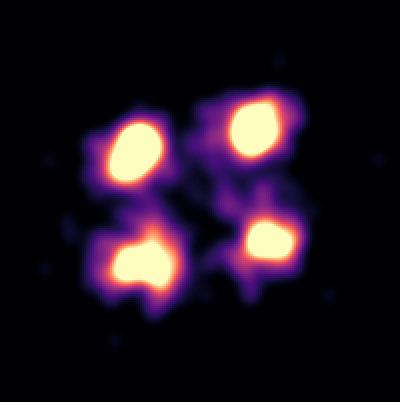
\includegraphics[width=\plotwidth]{figures/data/exp_counting/4bs_origami_1.png}
    \&
    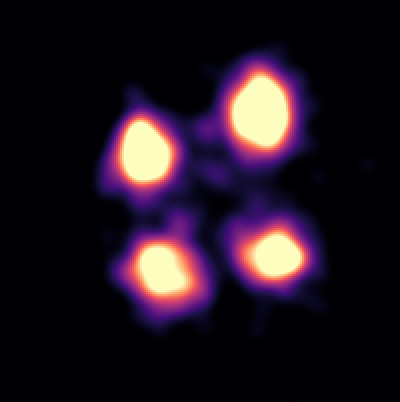
\includegraphics[width=\plotwidth]{figures/data/exp_counting/4bs_origami_2.png}
    \&
    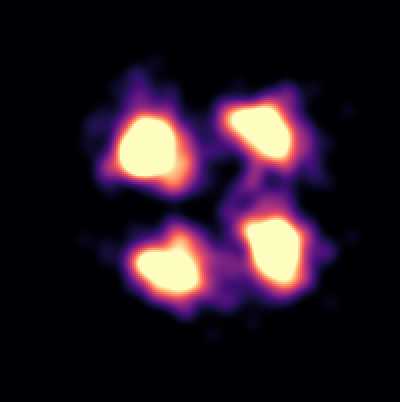
\includegraphics[width=\plotwidth]{figures/data/exp_counting/4bs_origami_3.png}
    \&
    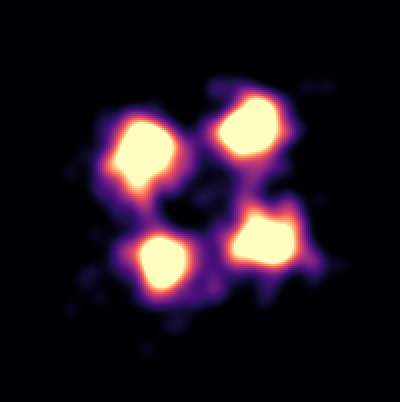
\includegraphics[width=\plotwidth]{figures/data/exp_counting/4bs_origami_4.png}
    \\
  };

  % scale bar
  \node[
    rectangle,
    minimum width=0.25\plotwidth, % images are 400px, 1/4 is 100px and that is 20nm
    fill=white,
    anchor=south east,
    inner sep=0pt,
    outer sep=2mm] (scalebar) at (samples-1-4.south east) {};
  \node[anchor=south,white] at (scalebar.center) {\tiny $20 \micrometer$};
\end{tikzpicture}
%
  \end{panel}
  \begin{panel}{(d)}{0.2\textwidth}
    \hspace{2mm}%
    \def\plotwidth{0.8\textwidth}%
    \def\plotheight{20mm}%
    \tikzsetnextfilename{exp_mean_probabilities_n1}%
\begin{tikzpicture}

  \pgfplotsset{every axis/.style={name=n1}}
  \def\posteriorcsv{figures/data/exp_counting/mean_probabilities.csv}
  \def\posteriorcol{n1_prob}
  \def\eps{0.001}%  skip bars for values below eps
\@ifundefined{noylabels}{}{
  \pgfplotsset{yticklabel=\empty}
  \pgfplotsset{ylabel=\empty}
}
\@ifundefined{noxlabel}{
  \pgfplotsset{xlabel=$n$}
}{
  \pgfplotsset{xlabel=\empty}
}
\begin{axis}[
  width=\plotwidth,
  height=\plotheight,
  scale only axis=true,
  enlarge x limits={abs=1.5},
  enlarge y limits=0,
  ymin=0,
  ymax=1,
  scaled ticks=false,
  ticklabel style={font=\tiny},
  xtick distance=1,
  axis background/.style={fill=white},
]

  \addplot+[
    ybar,
    bar width=1,
    mark=none,
    fill=posteriorcolor,
    fill opacity=0.6,
    draw=posteriorcolor,
    y filter/.expression={
      y < \eps ? nan : y
    },
  ] table [
    col sep=comma,
    y=\posteriorcol,
    x=n,
  ] {\posteriorcsv};

  \ifdefined\posteriorcolextra
    \addplot+[
      ybar,
      bar width=1,
      mark=none,
      fill=posteriorcolor!60!black,
      fill opacity=0.6,
      draw=posteriorcolor,
      y filter/.expression={
        y < \eps ? nan : y
      },
    ] table [
      col sep=comma,
      y=\posteriorcolextra,
      x=n,
    ] {\posteriorcsv};
  \fi

\end{axis}

  \node[anchor=south] at (n1.outer north) {origami with $\n=1$};

\end{tikzpicture}
%
  \end{panel}
  \begin{panel}{(e)}{0.2\textwidth}
    \hspace{2mm}%
    \def\plotwidth{0.8\textwidth}%
    \def\plotheight{20mm}%
    \tikzsetnextfilename{exp_mean_probabilities_n4}%
\begin{tikzpicture}

  \pgfplotsset{every axis/.style={name=n4}}
  \def\posteriorcsv{figures/data/exp_counting/mean_probabilities.csv}
  \def\posteriorcol{n4_prob}
  \def\eps{0.001}%  skip bars for values below eps
\@ifundefined{noylabels}{}{
  \pgfplotsset{yticklabel=\empty}
  \pgfplotsset{ylabel=\empty}
}
\@ifundefined{noxlabel}{
  \pgfplotsset{xlabel=$n$}
}{
  \pgfplotsset{xlabel=\empty}
}
\begin{axis}[
  width=\plotwidth,
  height=\plotheight,
  scale only axis=true,
  enlarge x limits={abs=1.5},
  enlarge y limits=0,
  ymin=0,
  ymax=1,
  scaled ticks=false,
  ticklabel style={font=\tiny},
  xtick distance=1,
  axis background/.style={fill=white},
]

  \addplot+[
    ybar,
    bar width=1,
    mark=none,
    fill=posteriorcolor,
    fill opacity=0.6,
    draw=posteriorcolor,
    y filter/.expression={
      y < \eps ? nan : y
    },
  ] table [
    col sep=comma,
    y=\posteriorcol,
    x=n,
  ] {\posteriorcsv};

  \ifdefined\posteriorcolextra
    \addplot+[
      ybar,
      bar width=1,
      mark=none,
      fill=posteriorcolor!60!black,
      fill opacity=0.6,
      draw=posteriorcolor,
      y filter/.expression={
        y < \eps ? nan : y
      },
    ] table [
      col sep=comma,
      y=\posteriorcolextra,
      x=n,
    ] {\posteriorcsv};
  \fi

\end{axis}

  \node[anchor=south] at (n4.outer north) {origami with $\n=4$};

\end{tikzpicture}
%
  \end{panel}

  \caption{
    \panelref{a, b} Experimental traces with super-resolution confirmed counts of one (a) and four (b), and \ours fits
    %
    \panelref{c} Super-resolution visualization of origamis made with four binding sites.
    %
    \panelref{d, e} Average \ours posterior distributions of 112 traces with a known $n$ of one (d) and 
    110 traces with a known $n$ of four (e)
  }
  \label{fig:results:experimental}
\end{figure*}


\subsection{Simulated Experiments}
% Simulated traces based on experimentally relevant parameters
Running \ours as a forward model, traces were generated for counts N=1 to 30
	(\figref{fig:results:sim_counting}a,b), with experimentally relevant parameters. 
	%
	Camera parameters were determined from an empirical calibration of the
	sCMOS camera (\parametersc: \camgain=2.17, \camoffset=4791, \camvar=774), 
	and kinetic (\parameterst: \pon=0.036, \poff=0.028), and emission parameters (\parameterse: \re=2.79, \rb=6.77) were determined through an
	initial experiment, and closely match those reported in literature \cite{stein_2021}.
	%
	Traces were generated for 4000 frames, corresponding to an imaging time of 14 minutes.

% priors were placed on camera parameters, but all others were uniform
While fitting, tight gaussian priors were placed on the camera parameters because these were empirically determined.
	%
	Flat uniform priors were place on the kinetic parameters, allowing the model to fit blinking rates without external bias.
	%
	Loose priors were placed on the emission parameters (\rb, \re) to prevent overcounting (discussed further in discussion). 
	% how we got these priors
	The prior on \rb can be experimentally determined by averaging the intensity of pixels immediately outside the spot ROI.
	The prior on \re was determined by first fitting a count of \n=1 to the trace.
	%
	Given the definitions of \pon and \poff, the most common transition from state $z$ will be to state $\z{} \pm 1$, a switch of a single emitter.
	It follows that the distribution of all observed $z$-states will be unimodal, and that whichever \z{}-state is the most common, 
	the second most common will be $\z{} \pm 1$. Therefore fitting $n=1$ will capture this transition 
	and as a result accurately estimate \re (the photon emission rate of a single emitter).
	%
	

% blinx can count!
\ours successfully fit simulated traces with counts up to N=30 (\figref{fig:results:sim_counting}c).
	%
	For N=10 and below, \ours fit the correct count, with a significantly higher likelihood than all other possibilities. 
	%
	Above N=10 the likelihood of other possible counts increased, but the posterior distribution remained centered on the correct count.
	%
	Importantly, \ours is able to fit the correct count,
	despite the fact that not every state is visited \ie the model is not just counting the number of peaks in the intensity histogram (\figref{fig:results:sim_counting}a,b).
	% blinx outperforms lbFCS, counting up to 30 
	This is a tripling in performance compared to lbFCS, which counted accurately up to N=7, but failed to estimate higher counts.
	% main limitation of lbFCS is estimation of the "step size" corresponding to r_e
	Upon further analysis, the main limitation of lbFCS is the estimation of the intensity of a single emitter, corresponding to $r_e$ in \ours. 
	%
	lbFCS relies on a histogram based method to determine this value, while \ours is able to jointly optimize this parameter with the others.
	%
	%If this value is first estimated by \ours, then supplied to lbFCS, performance is significantly rescued (SI Figure).

% Longer traces lead to better fits
Next, the effect of trace length on counting accuracy (\figref{fig:results:sim_counting}d) was investigated.
	%
	As expected accuracy increased and variance of the posterior distribution decreased, 
	as the number of observations increased.
	% Also notice a underestimation of count with low trace length
	Interestingly, for short trace lengths, \ours underestimated the true count. 
	%
	Underestimating more severely as the true count increased.
	% This is most likely due to the system only occupying a subset of all possible zs in this short time
	This is likely because only a subset of possible states were observed in this short time.

% there is a lower bound to SNR, below a specific SNR, model maximally overcounts
To investigate the effect of noise on counting ability, the variance of the readout noise \camvar was tuned to produce a 
	series of traces with differing SNR values. 
	%
	Because noise in our model is proportional to intensity, quantifying the SNR of a trace 
	is not trivial. 
	%
	For simplicity, here we define SNR as the difference in intensity between 
	the first two states (\z{0} and \z{1}) divided by the square root of the sum of the variances of both states. 
	%
	In effect this is the upper bound of SNR for a given trace. 
	%
	The base model, with experimentally measured \camvar corresponds to an SNR of 9. 
	%
	\ours shows similar performance down to an SNR as low as 4 (\figref{fig:results:sim_counting}e). 
	%
	Interestingly, at SNR's below 4, \ours estimates the count as 25, the highest \n tested, no matter the true count. 
	%
	This is due to the low probability of observing states far from the mean of our intensity model, and is further expanded on in the discussion. 


\subsection{Effect of kinetic parameters}
Next, we hypothesized that the performance of our model would depend on the true kinetic parameters of the system, 
and that a regime exists that maximizes our models counting ability, 

To sample this state space, traces were simulated from $\n=1$ to 20, with a range of kinetic parameters, 
while holding all other parameters constant.
	%
	Using the poisson distribution to convert from $k_{on}$ and $k_{off}$ to \pon and \poff,
	it was ensured that this range covered experimentally relevant kinetics from literature including:
	qPAINT: (\pon, \poff) = (0.006, 0.2) \cite{jungmann_2016} and lbFCS (0.02, 0.02) \cite{stein_2021}. 
	%
	Traces were fit, and the resulting posterior for all true counts reduced to the expected 
	square error(\figref{fig:results:campare_kinetics}a).
	%

The resulting heatmap can be divided into two clear regimes: $\pon < \poff$ and $\pon \geq \poff$.
	%
	In the first regime, where $\pon < \poff$ we see significant limitations to our models counting ability.
	%
	Further when \pon is significantly lower than \poff, our model looses almost 
	all ability to count and estimates $n=1$ or 2, regardless of the true $n$.
	%
	In contrast, in the second regime, where $\pon \geq \poff$ we see a heightened ability of or model, 
	and accurate counting up to $n=20$.
	%
	A clear difference between these 2 regimes can be seen in the distribution 
	of their hidden states \z (\figref{fig:results:campare_kinetics}a, insets).
	%
	When $\pon < \poff$, the distribution is shifted towards 0, and a majority 
	of the time is spent in the lowest two \z{}-states (\figref{fig:results:campare_kinetics}c). 
	In this regime, the true count becomes indistinguishable without prior information. 
	%
	When $\pon \geq \poff$, this distribution is centered, or even shifted towards $n$ 
	and a larger portion of the states are visited (\figref{fig:results:campare_kinetics}d). 
	%
	This provides ample information for the model to infer the correct $n$.
	
% Experimental
% Do we need to explain how DNA-PAINT works
In DNA-PAINT, the blinking rate is determined by the kinetics of single-stranded DNA binding,
which in turn are dependant on experimental conditions such as temperature and concentration, and sequence.
	%
	As a result, the kinetic parameters \pon and \poff of our model, are can be 
	tuned by adjusting the temperature and imager concentration.
	%
	Imaging DNA-origami with a known count of $\n=1$ at 25 C and an 
	imager concentration of 10 nM, we measured $\pon=0.028$ and $\poff=0.072$ 
	(\figref{fig:results:campare_kinetics}b).
	%
	Which places these conditions firmly in the poor counting 
	accuracy regime of $\pon < \poff$ (\figref{fig:results:campare_kinetics}a). % fix
	
In order to move to a more favorable kinetic regime, 
we increased the imager concentration and decreased the temperature.
	%
	Increasing imger concentration to 30 nM raised \pon to 0.071 and 
	decreasing temperature to 13 C decreased \poff to 0.037 
	(\figref{fig:results:campare_kinetics}b).
	%
	The effects of temperature and concentration were largely independent 
	of one another providing precise control over the kinetic parameters. % cite jungmann paper
	%
	We also observed a significant decrease in SNR with decreasing temperature, 
	and with increasing concentration. 
	%
	This was an expected side effect of increasing concentration, as more imager would increase \rb.
	%
	But the effect of temperature on SNR was surprising. 
	We hypothesize that this is due to the stabilization partial 
	binding between imager and docker strands at low temperatures.
	%
	Accounting for both the increase in counting accuracy and the decrease 
	in SNR, imaging conditions of 20 nM and 13 C were chosen as optimal.

\subsection{qPAINT Kinetic Regime}
% qPAINT operates in a different kinetic regime that lbFCS
qPAINT is based on an accurate measure of the average dark time between blinking events. 
	%
	As a result, this method operates in an entirely different kinetic regime than lbFCS, where blinking 
	events are short and infrequent (\figref{fig:results:qpaint_counting}a,b).
	% this presents challenges to blinx
	This regime presents a challenge to \ours. 
	%
	If the only states ever observed are z=0 or 1 (off or on), there is not enough information in the system to estimate count without prior knowledge.
	% qPAINT relies on a calibration of kinetics
	qPAINT, faces the same limitation, and relies on a calibration of the blinking kinetics of a single binding site.
	% However, blinx is fully Bayesian and we can overcome these challenges by tightening priors
	\ours, as a fully Bayesian model can easily incorporate the same calibration as priors of the kinetic parameters
	and once again accurately count up to N=30 (\figref{fig:results:qpaint_counting}c).

% qPAINT undercounts but blinx does not
Due to the stochastic nature of blinking, multiple binding sites can blink at the same time, which becomes increasingly likely at higher counts.
	%
	This is not compatible with the qPAINT assumption of well separated, single binding-site blinking events, 
	and as a result, qPAINT begins to underestimate molecular count, (especially noticeable above N=20, (\figref{fig:results:qpaint_counting}c)). 
	% blinx avoids this problem
	The blinking of multiple binding sites at the same time point, 
	is compatible and accounted for in the transition model of blinx 
	and as a result, blinx accurately estimates the count even at higher N.
	

\subsection{Experimental Counting}
% briefly describe experimental setup
To experimentally validate the counting performance of \ours, DNA-Origami, which allows fine control over the number of emitters, was used.
	% Why DNA origami
	DNA-Origamis were designed containing 1 and 4 DNA-PAINT docker strands, spaced in a grid 20 \nanometer apart. 
	%
	This distance was specifically chosen, so that the true number of docker strands could be visually confirmed through super-resolution post-processing.
	%
	Incorporation efficiency is roughly 80 percent for each docker site \cite{strauss_2018}, so only a fraction of the origamis were expected to contain all 4 dockers. 
	% 
	Origamis were first imaged at 13 C, low laser power, and 20 nM imager concentration to collect traces for counting with \ours (\figref{fig:results:experimental}a,b).
	%
	Then the system was allowed to warm to 25C, a buffer exchange performed and new imager added at 10 nM, and the origamis were imaged again at high laser power,
	and post-processed to obtain super-resolution ground truth (\figref{fig:results:experimental}c).
	%
	Only origamis that had a visual count matching the designed count (1 or 4) were selected for analysis with \ours.

Of 131 traces with a known count of 1, \ours correctly counted 112 (85\%) and the maximum estimated count was 3 (1/131) (\figref{fig:results:experimental}e).
	%
	For the traces with a known count of 4, 71/110 (65\%) were correctly identified as 4, and 103/110 were identified as between 3 and 5.
	%
	% A more detailed analysis of wrongly counted traces is found in the SI.
	%
	Importantly, no filtering or preprocessing was done on the measured traces, and many of the incorrect counts were due to low trace SNR. % quantify this??
